

%!TEX root = /Users/stevenmartell/Documents/CURRENT PROJECTS/iSCAM-trunk/fba/BC-herring-2011/PRESENTATION/BC-Herring-2011.tex
%%%   %%%   %%%   %%%   %%%   %%%   %%%   %%%   %%%   %%%   %%%   %%%   %%%   %%%   
%% Outline for Part I
%% Introduction:
%% Analytical approach:
%% 
%%%   %%%   %%%   %%%   %%%   %%%   %%%   %%%   %%%   %%%   %%%   %%%   %%%   %%%   
%%%%%%%%%%%%%%%%%%%%%%%%%%%%%%%%%%%%%%%%%%%%%%%%%%%%%
%%%%%%%%%%%%%%%%%%%%%%%%%%%%%%%%%%%%%%%%%%%%%%%%%%%%%
\begin{frame} % (fold)
	\frametitle{Moving towards the sustainable fisheries framework.} 
	\begin{block}
		{Overview} 
		\begin{itemize}
			\item Review of the HCAM model in June 17-18, 2010. 
			\begin{itemize}
				\item Model parameterization of $q$. 
				\item Parametrization of $q$, $M$, and selectivity is confounded. 
			\end{itemize}
			\item Development of a new integrated Statistical Catch Age Model (\iscam). 
			\item Data, assumptions and Analytical methods. 
			\item Outstanding issues. 
		\end{itemize}
	\end{block}
\end{frame}




%%%%%%%%%%%%%%%%%%%%%%%%%%%%%%%%%%%%%%%%%%%%%%%%%%%%%
%%%%%%%%%%%%%%%%%%%%%%%%%%%%%%%%%%%%%%%%%%%%%%%%%%%%%
\section{Introduction} % (fold)
\label{sec:introduction}

%
\begin{frame}
	\frametitle{Introduction} 
	\begin{itemize}
		\item Current harvest control rule for BC herring: 
		\begin{itemize}
			\item Cuttoffs set at 0.25 $B_0$ 
			\item 20\% exploitation rate 
			\item Estimates of $B_0$ were last updated in 1996. 
		\end{itemize}
		\item HCAM model assumed $q=1$ for the dive survey data. 
		\item Natural mortality is modelled as a random-walk. 
		\item Gill net selectivity is a function of weight-at-age. 
	\end{itemize}
\end{frame}

%
\begin{frame}
	\frametitle{Harvest Strategy Compliant with Precautionary Approach} 
	\begin{figure}
		[htbp] \centering 
		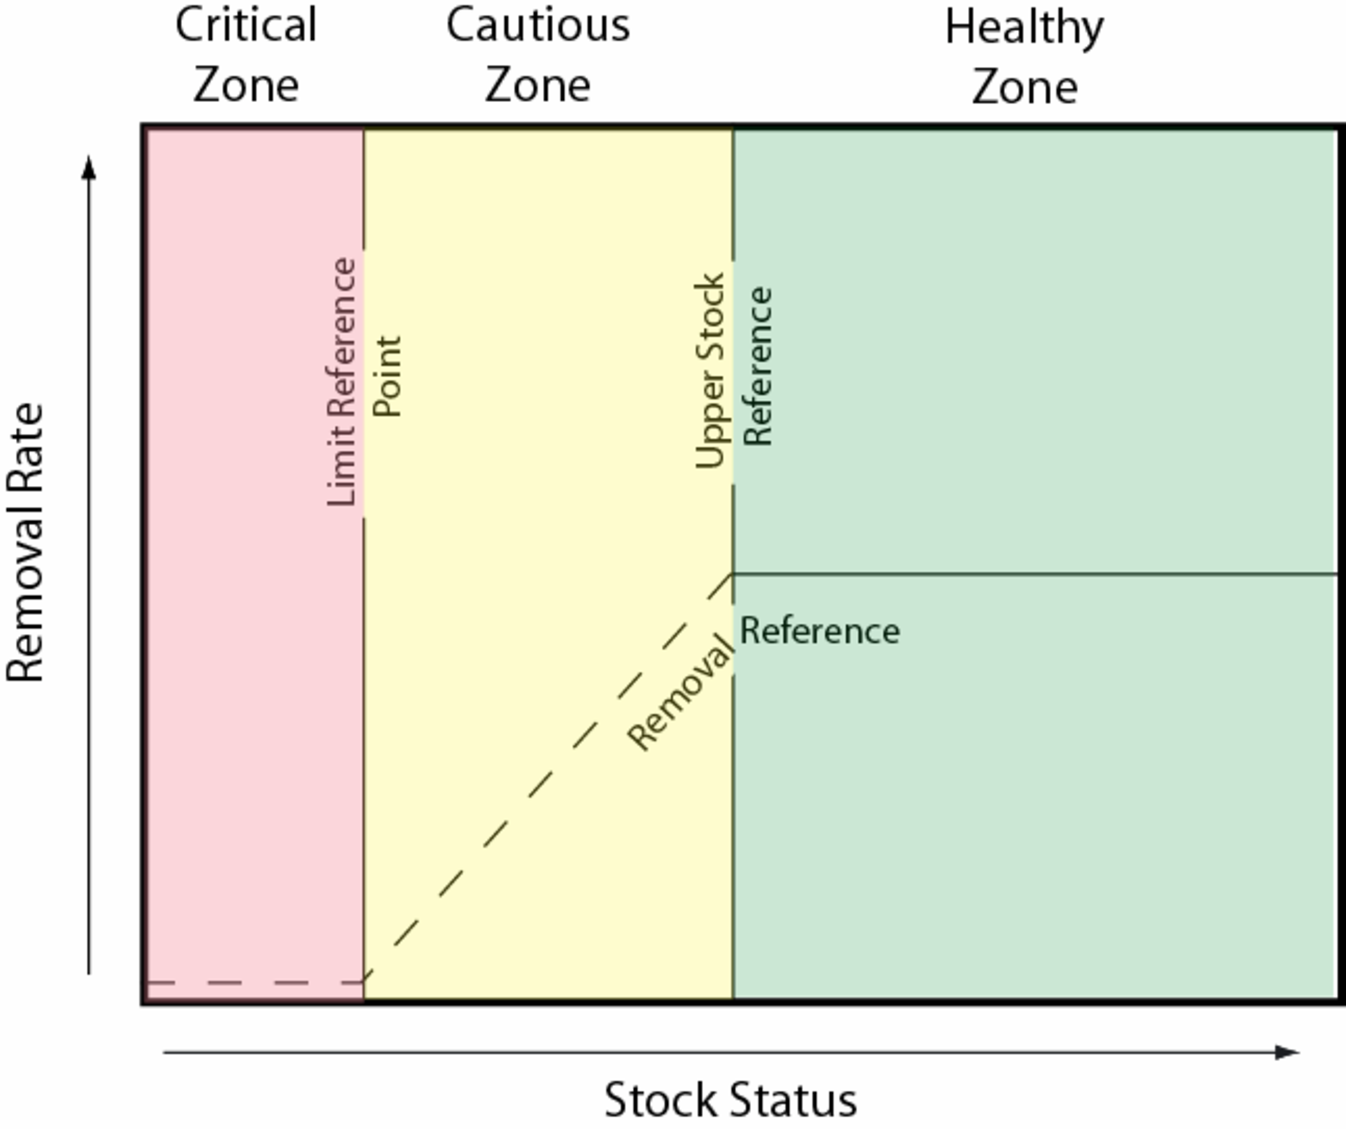
\includegraphics[width=0.7
		\textwidth]{SSF} \caption{Fisheries management framework consistent with a precautionary approach.} \label{fig:label} 
	\end{figure}
\end{frame}

%
\begin{frame}[allowframebreaks]
	\frametitle{Key elements for the new framework} 
	\begin{block}
		{Reference points} 
		\begin{itemize}
			\item Limit Reference Point (LRP) \& Upper Stock Reference (USR) requires knowledge of stock productivity and population scale. 
			\item Removal Rate requires knowledge of stock productivity. 
			\item MSY-based reference points require \textit{a priori} allocation to different gears. 
		\end{itemize}
	\end{block}
	\begin{block}
		{Risk \& Decision making} 
		\begin{itemize}
			\item Onus on being able to reliably determine stock status (informative data). 
		\end{itemize}
	\end{block}
\end{frame}

%
\begin{frame}[allowframebreaks]
	\frametitle{Herring Stock Assessment Model Review} 
	\begin{block}
		{Summary of Panel Recommendations} 
		\begin{itemize}
			\item Panel concluded that $q_2=1$ was inappropriate. 
			\item CUTOFFS can be fixed or annually estimated (should be updated if management objective is 25\% $B_0$) 
			\item A model based approach to estimating $B_0$ and $B_{MSY}$ is appropriate. 
			\item Recruitment variation should be estimated within the model rather than fixing it at a pre-specified level. 
			\item Issues regarding estimating selectivity vs. availability should be explored (data is limited to estimate availability). 
			\item Science advice should be risk neutral. 
			\item MSE should explore elements of the Sustainable Fisheries Framework (i.e., ensure that $B_t>0.4B_{MSY}$ with 95\% certainty over two generations.) 
			\item ... 
		\end{itemize}
	\end{block}
\end{frame}
% section introdution (end)




%%%%%%%%%%%%%%%%%%%%%%%%%%%%%%%%%%%%%%%%%%%%%%%%%%%%%
%%%%%%%%%%%%%%%%%%%%%%%%%%%%%%%%%%%%%%%%%%%%%%%%%%%%%
\section{inputdata} % (fold)
\label{sec:inputdata}

%
\begin{frame}
	{Input data} The input data for \iscam\ is the same as HCAM: 
	\begin{itemize}
		\item Catch by gear, 
		\item Spawn survey index, 
		\item Age-composition data for all gears, 
		\item Empirical weight-at-age data. 
	\end{itemize}
\end{frame}

% section inputdata (end)




%%%%%%%%%%%%%%%%%%%%%%%%%%%%%%%%%%%%%%%%%%%%%%%%%%%%%
%%%%%%%%%%%%%%%%%%%%%%%%%%%%%%%%%%%%%%%%%%%%%%%%%%%%%
\section{analyticalMethods} % (fold)
\label{sec:analyticalmethods}
%
\begin{frame} {Analytical methods} 
	
	\begin{block}
		{Integrated Statistical Catch Age Model (\iscam)}
		\begin{itemize}
			\item The model is based on a statistical catch-age framework first developed by \cite{fournier1982general}.
			
			\item Flexible options for modelling selectivity, natural mortality, \& survey catchability.
			
			\item Integrated framework: joint estimation of policy parameters (e.g., reference pionts).
			\item Bayesian implementation... 
		\end{itemize}
	\end{block}
\end{frame}
%
\begin{frame}[t]\frametitle{Assumptions}
	\begin{itemize}
		\item<+-> Observation errors in catch is known
		\item<+-> Survey $q$ is proportional
	\end{itemize}
\end{frame}
% section analyticalmethods (end)
